\section{Aufgabenstellung}
\label{sec:aufgabenstellung}

Wie in der Einleitung erwähnt, behandelt diese Arbeit die Entwicklung einer
Software, welche bei einem praktischen Test der Sensorknoten in Verbindung mit
dem Referenzsystem entstandene Pfaddaten zusammenführt und für den Nutzer
aufwertet. Die Software trägt den Namen Pathcompare.
Im folgenden wird die Abgrenzung von Pathcompare zum 
Referenzsystem beschrieben. Dazu wird zunächst der Aufbau und die grundlegende
Funktionsweise des Referenzsystems erläutert.

\subsection{Referenzsystem}
\label{sub:roboter}

Im Referenzsystem steht auf Ebene der Hardware ein mobiler Roboter. Dieser hat
das Ziel, sich genau zu lokalisieren, um Referenzwerte für die montierten,
mobilen Sensorknoten zu liefern. Da er sich während der Testfahrten indoor
bewegt, kann er für seine Lokalisierung keine satellitengestützten
Lokalisierungssysteme wie GPS verwenden, aus den in der Einleitung genannten
Gründen. 

Zwei weitere Ansätze die in Betracht gezogen wurden, um die Bewegung
des Roboters nachzuvollziehen und somit Positionsdaten zu gewinnen, sind:

\begin{itemize}
  \item Inertial Navigation
  \item Odometrie
\end{itemize}

Bei der inertial Navigation wird mithilfe von Beschleunigungs- und
Gyromessungen auf die ausgeführte Bewegung geschlossen. Diese Messungen lassen
sich durch \gls{MEMS}, die in einer 
\gls{IMU} zusammengefasst werden, durchführen.
MEMS werden in großen Stückzahlen produziert und sind kostengünstig.
Typischerweise sind aber die Messungen, auch bei Stillstand, durch Jitter belastet.
Dieser kann zwar durch geeignete Filter geglättet werden, lässt sich allerdings
nicht ganz ausschließen. Auf längere Strecken entsteht durch die Aufsummierung
der Fehler eine zunehmende Differenz zwischen geschätzer und tatsächlicher
Position. Dieser Effekt wird als Drift bezeichnet.

Bei der Odometrie werden die Antriebsdaten ausgewertet, um auf die Bewegung
des Roboters zu schließen. Geht man davon aus, dass der Untergrund auf dem der
Roboter fährt für dessen Räder geeignet ist und die Räder nicht wegen
beispielsweise mangelnder Bodenhaftung stark durchdrehen, so kann sie auf
kurzen Strecken sehr genaue Abschätzungen liefern. Allerdings ist auch eine
Odometriemessung stets mit einem Fehler behaftet. Dieser Fehler summiert sich
über die Zeit auf und die geschätzte Position weicht immer weiter von der
tatsächlichen ab. Man hat also auf längeren Strecken ebenfalls mit einem Drift
zu rechnen.

Beide Methoden haben gemeinsam, dass sie unabhängig von Informationen aus der
Umgebung des Roboters arbeiten. Somit können sie allerdings den beschriebenen
Drift in der Lokalisierung niemals korrigieren, da sie nicht die Positions auf
Plausibilität mit der Umgebung abgleichen.  Für das Referenzsystem ist Drift
aber nicht akzeptabel. Aus diesem Grund erfasst der Roboter Abstände zu
Hindernissen seiner Umgebung mithilfe einer \textit{Microsoft Kinect}
\footnote{\url{http://www.xbox.com/de-DE/kinect}}. Die
Kinect erstellt mithilfe eines, im infrarot Bereich gestrahltem, optischen
Musters ein Tiefenbild.  Die Reichweite liegt dabei bei maximal 10 Meter
Entfernung bei einem Blickwinkel von ca. $59^{\circ}$.
%TODO Quelle anbringen
Tests haben gezeigt, dass die Genauigkeit der Tiefenmessung mit zunehmender
Entfernung abnimmt. Im Nahbereich von zwei Metern ermöglicht die Kinect eine überraschend präzise
Distanzmessung. Die Genauigkeit liegt dabei im Zentimeterbereich.  Außerdem verfügt der Roboter
über eine Karte der Testumgebung. Diese Karte in Kombination mit der
Microsoft Kinect ermöglicht während einer Testfahrt eine Lokalisierung
durch folgende grundlegende Schritte durchzuführen:

\begin{enumerate}
  \item Abschätzung der derzeitigen Position und Ausrichtung durch Odometrie
  \item Abgleich mit Karte und Korrektur der Pose
\end{enumerate}

Zum Abtasten der Umgebung hätte alternativ auch ein Laserscanner gewählt werden
können, welcher hohe Reichweite mit hoher Genauigkeit kombiniert. Dies wäre
aber mit hohen Anschaffungskosten verbunden gewesen. Mit dem Ziel ein günstiges
Referenzsystem zu schaffen, wurde schlussendlich ein sogenannter
\textit{TurtleBot} gebaut. Dies ist ein von \textit{WillowGarage}
spezifizierter low-cost Roboter.
%TODO TurtleBot specs referenzieren?
Im Kern besteht dieser aus einem \textit{Roomba} Staubsaugerroboter von
\textit{iRobot}, einer \textit{Microsoft Kinect} und einem Tragegerüst. 
\footnote{\url{http://www.willowgarage.com/turtlebot/specs}}
Das Tragegerüst dient als Abstellfläche für einen Laptop und bietet im
Anwendungsfall des Referenzsystems Platz zum Montieren der Sensorknoten.

Details zum Roboter und damit verbundener Software werden 
innerhalb einer separaten Bachelorarbeit, ebenfalls im Rahmen der
Entwicklung des Referenzsystems, ausführlich erarbeitet.

Zusammenfassend kann man bezüglich des Referenzsystems feststellen, dass zum autonomen Fahren
Programme des ROS genutzt werden. Außerdem wurde eine Software implementiert,
die den Roboter vorgegebene Wegpunkte abfahren lässt und dabei gesammelte
Lokalisierungsdaten innerhalb von ROS bereitstellt. Genauer wird im
Kapitel Implementierung auf die Funktionsweise von ROS eingegangen, da
Pathcompare mit ROS interagiert.

\subsection{Ziele Pathcompares}

Bei der Entwicklung von Pathcompare wurden folgende Ziele verfolgt:

\begin{enumerate}
  \item Zusammenführen der Pfaddaten an einem Ort
  \item Abweichung zum Referenzpfad bestimmen
  \item Anpassungsfähig und erweiterbar
\end{enumerate}

Der erste Punkt bezieht sich auf die durch wiederholte Lokalisierung des
Roboters und der Sensorknoten anfallenden Pfaddaten. Ziel ist es, diese bei
Durchführung eines Tests zu vereinen und einem Tester Informationen bezüglich
der Daten zu visualisieren. Unter dem zweiten Punkt wird die wichtigste dabei
ermittelte Information angeführt, nämlich die Bestimmung des Abstands eines
Pfads zum Referenzpfad des Roboters. Zusätzlich, soll wie unter Punkt drei
aufgeführt, Pathcompare anpassbar und erweiterbar für geänderte
Testanforderungen sein. Wie die Ziele realisiert wurden, wird im Abschnitt
Implementierung genauer beleuchtet.

\subsection{Überblick Testdurchführung}

In \autoref{fig:referencetopo} wird ein Überblick auf die Komponenten gegeben,
die an einer Testdurchführung beteiligt sind und wie diese miteinander in
Beziehung stehen.

\begin{figure}[t]
  \begin{center}
    \fbox{\includegraphics{./graphics/referencetopo}}
  \end{center}
  \caption{Struktur des Referenzsystems während der Testausführung}
  \label{fig:referencetopo}
\end{figure}

Erkennbar sind dabei zum einen die mobilen Sensorknoten, welche in das \gls{WSN} integriert sind.
Diese sind am TurtleBot Roboter befestigt. Die Sensorknoten und der Roboter
sind dabei mit einer als ``Node'' bezeichneten Komponente versehen. Diese dient zur
Anbindung an das ROS. Während der Roboter direkt druch ROS betrieben wird, sind
für die mobilen Sensorknoten zusätzliche Softwareadapter nötig, welche die
Anbindung zu ROS vornehmen. Die Verbindung der Komponenten erfolgt dabei über ein
Netzwerk, wobei der Roboter nach außen über WLAN kommuniziert, um ihn nicht in seiner
Mobilität einzuschränken.
